\section*{Exercise 2 - Semi-implicit schemes}

\textbf{a} The grid used to discretize \autoref{eq:SWE} can be seen in \autoref{fig:grid}. Discretizing \autoref{eq:u} and \autoref{eq:h} (we do not discretize \autoref{eq:v} since it is trivial) we obtain: 
\begin{subequations}
\begin{empheq}[left=\empheqlbrace]{align}
    \frac{u_{i}^{n+1}-u_{i}^{n-1}}{2 \Delta t} &= -g \left[\left(1-\beta\right)\frac{h_{i+1}^{n+1}-h_{i}^{n+1}}{\Delta x}+\beta\frac{h_{i+1}^{n-1}-h_{i}^{n-1}}{\Delta x}\right] \\
    \frac{h_{i}^{n+1}-h_{i}^{n-1}}{2 \Delta t} &= -H \left[(1-\beta)\frac{u_{i}^{n+1}-u_{i-1}^{n+1}}{\Delta x}+\beta\frac{u_{i}^{n-1}-u_{i-1}^{n-1}}{\Delta x}\right],
\end{empheq}
\label{eq:disc}
\end{subequations}
where we know that the implicit parameter is $\beta=0.5$.

\begin{figure}[H]
    \centering 
    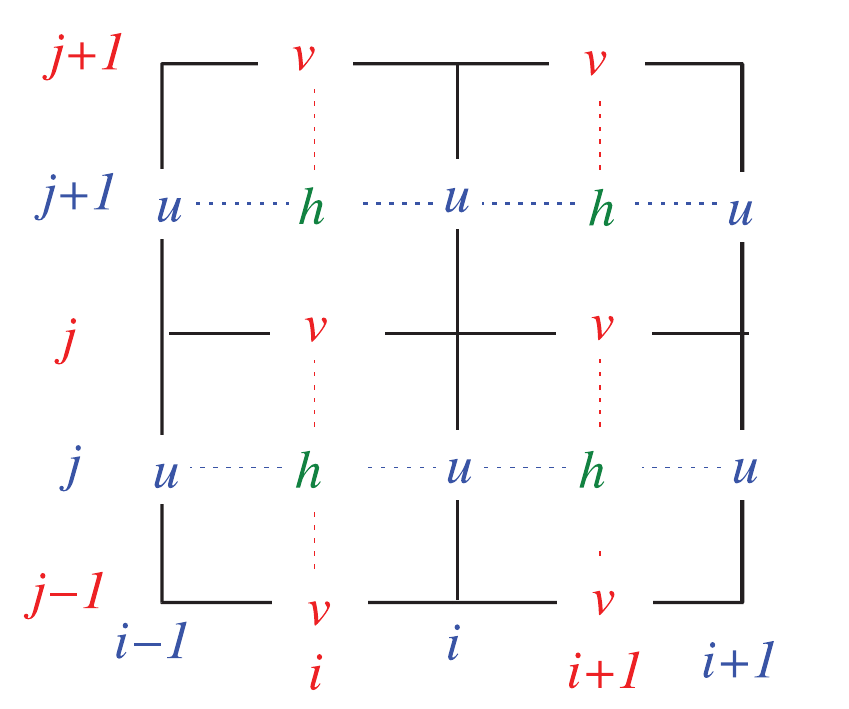
\includegraphics[width=0.5\textwidth]{Figures/cgrid.png}
    \caption{This figure displays the Arakawa c-grid.}
    \label{fig:grid}
\end{figure}

\textbf{(b)} To evaluate the stability \autoref{eq:disc} one has to use the Von Neumann method as 
\begin{equation*}
    \begin{pmatrix}
        u_{i}^{n} \\
        h_{i}^{n}
    \end{pmatrix} = 
    \begin{pmatrix}
        u_0 \\
        h_0
    \end{pmatrix}
    e^{\mathfrak{I}\left(ik\Delta x - \omega_D n \Delta t\right)}
    \implies
    \begin{aligned}
        u_{i}^{n\pm1} &= \lambda^{\pm1} u_{i}^n \\
        u_{i\pm1}^{n} &= e^{\pm\mathfrak{I}k\Delta x} u_{i}^n 
    \end{aligned}
    \quad \text{and} \quad
    \begin{aligned}
        h_{i}^{n\pm1} &= \lambda^{\pm1} h_{i}^n \\ 
        h_{i\pm1}^{n} &= e^{\pm\mathfrak{I}k\Delta x} h_{i}^n
    \end{aligned}
\end{equation*}
where $\mathfrak{I}$ is the imaginary unit, $k$ is the wavenumber nad $\lambda$ is the relative step size in time. 

This transforms \autoref{eq:disc} into
\begin{align*}
    \left(\lambda -\lambda^{-1}\right)u_{i}^{n} &= -\frac{g \Delta t}{\Delta x} \left(\lambda e^{\mathfrak{I}k\Delta x}-\lambda +\lambda^{-1}e^{\mathfrak{I}k\Delta x}-\lambda^{-1}\right)h_{i}^{n} \\
    \left(\lambda -\lambda^{-1}\right) h_{i}^{n} &= -\frac{H\Delta t}{\Delta x} \left(\lambda -\lambda e^{-\mathfrak{I}k\Delta x}+\lambda^{-1  }-\lambda^{-1}e^{-\mathfrak{I}k\Delta x}\right)u_{i}^{n}.
\end{align*}
Combining the two equations above and using the Courant number $\mu=\tfrac{c\Delta t}{\Delta x}$, where $c=\sqrt{gH}$ gives 
\begin{align*}
    \left(\lambda -\lambda^{-1}\right)^2 &= \mu^2 \left(\lambda e^{\mathfrak{I}k\Delta x}-\lambda +\lambda^{-1}e^{\mathfrak{I}k\Delta x}-\lambda^{-1}\right) \left(\lambda -\lambda e^{-\mathfrak{I}k\Delta x}+\lambda^{-1}-\lambda^{-1}e^{-\mathfrak{I}k\Delta x}\right) \\
    \begin{split}
    &=\mu^2 \left( \lambda^2e^{\mathfrak{I}k\Delta x}-\lambda^2+e^{\mathfrak{I}k\Delta x}-1    -\lambda^2+\lambda^2e^{-\mathfrak{I}k\Delta x}-1+e^{-\mathfrak{I}k\Delta x}\right. \\
        &\quad \quad \quad \left. 
    e^{\mathfrak{I}k\Delta x}-1+\lambda^{-2}e^{\mathfrak{I}k\Delta x}-\lambda^{-2} -1+e^{\mathfrak{I}k\Delta x}-\lambda^{-2}+\lambda^{-2}e^{-\mathfrak{I}k\Delta x}\right).
    \end{split} \\
    &= \mu^2  \left[\lambda^2\left(2\cos(k\Delta x)-2\right)+2\left(2\cos(k\Delta x)-2\right)+\lambda^{-2}\left(2\cos(k\Delta x)-2\right)\right] \\
    & = 2\mu^2\left[\cos(k\Delta x)-1\right]\left(\lambda^2+2+\lambda ^{-2}\right) \\
    & = 2\mu^2\left[\cos(k\Delta x)-1\right]\left(\lambda+\lambda ^{-1}\right)^2.
\end{align*}
Now one can use the fact that $\left(\lambda -\lambda^{-1}\right)^2=\left(\lambda +\lambda^{-1}\right)^2-4$ together with the fact that $1-\cos(2\theta)=2\sin^2(\theta)$ and obtain
\begin{align*}
    \frac{\left(\lambda +\lambda^{-1}\right)^2-4}{\left(\lambda +\lambda^{-1}\right)^2} 
    & = -4\mu^2\sin^2\left(\frac{k\Delta x}{2}\right) \\
    1-\frac{4}{\left(\lambda +\lambda^{-1}\right)^2}&=-4\mu^2\sin^2\left(\frac{k\Delta x}{2}\right) \\
    \left(\lambda +\lambda^{-1}\right)^2&=\frac{4}{1+4\mu^2\sin^2\left(\frac{k\Delta x}{2}\right)}=B^2.     
\end{align*}
Where $B$ is a real positive number in the range $B\in\left[2\sqrt{\tfrac{1}{1+4\mu^2}},2\right]$, where $0<\sqrt{\tfrac{1}{1+4\mu^2}}<1$. One can thus also state that $B\in\left(0,2\right]$ Solving this second order equation in $\lambda$ gives:
\begin{align*}
    \lambda^2-B\lambda+1=0 \implies \lambda_{1,2}=\frac{B}{2}\pm\sqrt{\frac{B^2}{4}-1}
\end{align*}
Now we obtain two cases, where the root is imaginary or real. 
\begin{itemize}
    \item If $\frac{B^2}{4}-1<0$ we have an imaginary solution: This would yield that 
    \begin{equation*}
        \lambda_{1,2}=\frac{B}{2}\pm \mathfrak{I}\sqrt{1-\frac{B^2}{4}}.
    \end{equation*}
    We thus obtain a norm of 
    \begin{equation*}
        \lambda^2=\frac{B^2}{4}+ {1-\frac{B^2}{4}}=1.
    \end{equation*}
    Thus if $\frac{B^2}{4}-1<0$ (or $B^2<4$) then we have an unconditionally stable solution!
    \item The real solution occurs when $\frac{B^2}{4}-1>0$, or in other words $B^2\geq4$. One can note that we have the limit $B^2$ cannot exceed the value of 2, but can obtain the value when the sin-term goes to zero. Therefore this occurs if and only if $B=2$, which would yield 
    \begin{equation*}
        \lambda = 1\pm0=1,
    \end{equation*}
    which also is unconditionally stable!
\end{itemize}
\begin{answer}
    The scheme is unconditionally stable for any choice of Courant number. However, the solution does obtain imaginary time steps which indicate oscillatory behaviour. Furthermore, the oscillatory behaviour is independent of the of Courant number, and will thus always exist. However this is probably due to the nature of the shallow water equations having a wave solution. Observing the numerical solution in \autoref{fig:}, one can see normal behaviour the solution.
\end{answer}

\begin{figure}[H]
    \centering    
    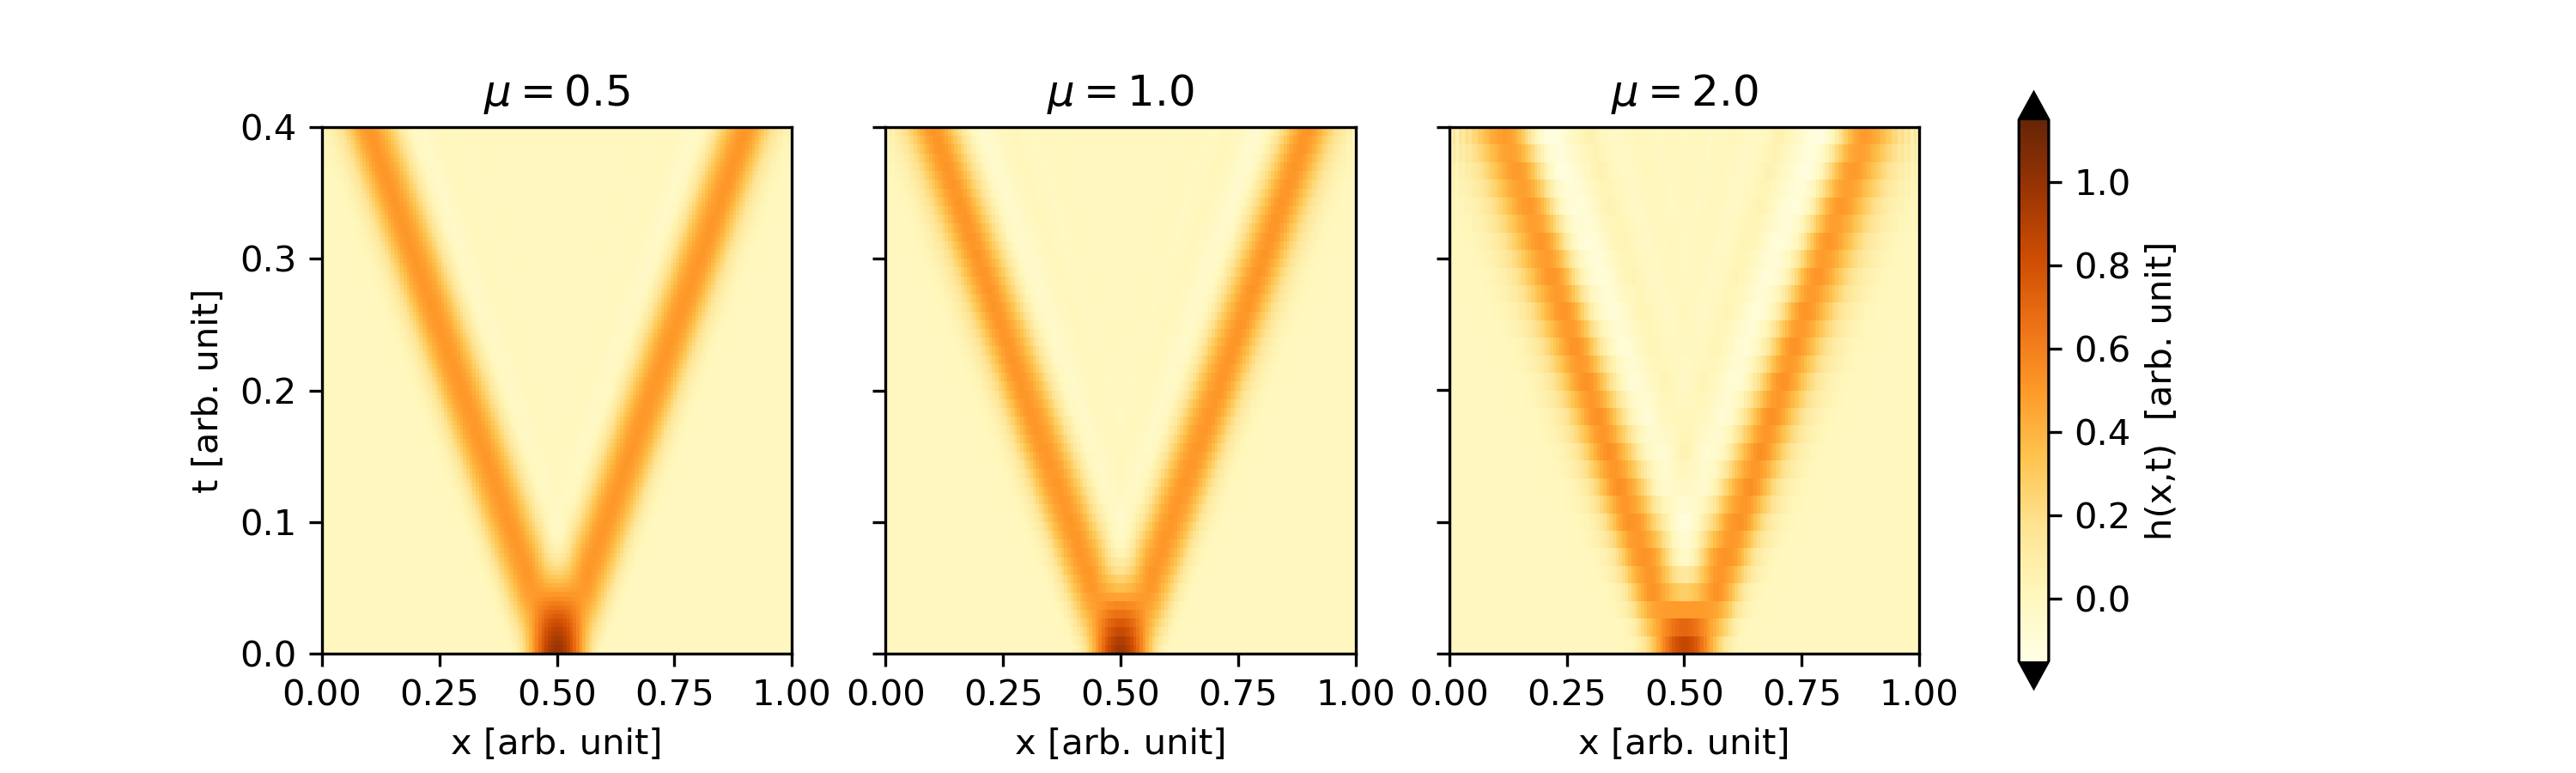
\includegraphics[width=\textwidth]{Figures/sol.png}
    \caption{This figure displays the real solution when $g=1$ and $H=1$, and the initial condition is a localised cosine-pulse. The solution was obtained through the use of the matrix-method. }
    \label{fig:}
\end{figure}



